% This is a LaTeX input file.
%
% A '%' character causes TeX to ignore all remaining text on the line,
% and is used for comments like this one.

\documentclass[a4paper]{article}      % Specifies the document class
                             % The preamble begins here.
\title{Hodges--Lehmann median differences between exponential subpopulations}  % Declares the document's title.
\author{Roger B. Newson}      % Declares the author's name.
\date{12 October, 2008}      % Deleting this command produces today's date.

\usepackage{graphics}
\usepackage{hyperref}

%
% Set margins
% (which are explained in Figure C3 of LaTeX User's Guide
% and which CAN BE RESET BY EDITORS AT ANY TIME AS FAR AS I CARE!!!!!!!!
% - RBN.)
%
\setlength{\topmargin}{-0.5in}
%\setlength{\headsep}{0.25in}
\setlength{\oddsidemargin}{0in}
\setlength{\evensidemargin}{0in}
\setlength{\textwidth}{6.5in}
\setlength{\textheight}{10in}

%
% Set page style (headers and footers)
%
\pagestyle{myheadings}
\markboth{\textit{Hodges--Lehmann median differences between exponential subpopulations}}
{\textit{Hodges--Lehmann median differences between exponential subpopulations}}

\begin{document}             % End of preamble and beginning of text.

\maketitle                   % Produces the title.

\section{Formulas}

\def\Ymin{Y_{\rm min}}
\def\Ymaj{Y_{\rm maj}}
\def\sigmamin{\sigma_{\rm min}}
\def\sigmamaj{\sigma_{\rm maj}}
\def\Pr{{\rm Pr}}
Suppose that $\Ymin$ and $\Ymaj$ are scalar random variables, sampled independently from 2 exponential subpopulations,
with means (and therefore also standard deviations) equal to
$\sigmamin$ and $\sigmamaj$ respectively, where $\sigmamin \le \sigmamaj$.
Given $q \in (0,1)$, we aim to define formulas for the $100q$th percentile differences $\xi_q ( \Ymaj - \Ymin )$,
defined as solutions in $\theta$ to the equation
\begin{equation}
\Pr \left\{ \Ymaj - \Ymin \le \theta \right\} = q .
\label{eq:eqseq1}
\end{equation}
In particular, we aim to define a formula for $\xi_{0.5} ( \Ymaj - \Ymin )$,
known as the Hodges--Lehmann median difference between $\Ymaj$ and $\Ymin$.
(See Hodges and Lehmann (1963) and Lehmann (1963).)

The variables $\Ymaj$ and $\Ymin$ have constant hazard rates $\sigmamaj^{-1}$ and $\sigmamin^{-1}$, respectively.
It follows that
\begin{equation}
\begin{array}{rcl}
\Pr \left\{ \Ymaj - \Ymin < 0 \right\} &\quad = \quad& \sigmamaj^{-1} / ( \sigmamaj^{-1} + \sigmamin^{-1} ) , \\
\Pr \left\{ \Ymaj - \Ymin > 0 \right\} &\quad = \quad& \sigmamin^{-1} / ( \sigmamaj^{-1} + \sigmamin^{-1} ) ,
\end{array}
\label{eq:eqseq2}
\end{equation}
and that the conditional distribution of $\Ymin - \Ymaj$ given that $\Ymaj < \Ymin$,
and the conditional distribution of $\Ymaj - \Ymin$ given that $\Ymin < \Ymaj$,
are both exponential, with means $\sigmamin$ and $\sigmamaj$, respectively.
It follows that, for any real $\theta$,
\begin{equation}
\Pr \left\{ \Ymaj - \Ymin \le \theta \right\} \quad = \quad \left\{
\begin{array}{ll}
{ \sigmamaj^{-1} \over {\sigmamaj^{-1} + \sigmamin^{-1}} } \exp ( \theta/\sigmamin ),
  & \mbox{if $\theta < 0$,} \\
{ \sigmamaj^{-1} \over {\sigmamaj^{-1} + \sigmamin^{-1}} } \quad + \quad { \sigmamin^{-1} \over {\sigmamaj^{-1} + \sigmamin^{-1}} } \left[ 1 - \exp (- \theta/\sigmamaj) \right] ,
  & \mbox{if $\theta \ge 0$.}
\end{array}
\right.
\label{eq:eqseq3}
\end{equation}
Therefore, given $q \in (0,1)$, the 100$q$th percentile difference $\xi_q ( \Ymaj - \Ymin )$ is a solution in $\theta$ to the equation
\begin{equation}
q \quad = \quad \left\{
\begin{array}{ll}
{ \sigmamaj^{-1} \over {\sigmamaj^{-1} + \sigmamin^{-1}} } \exp ( \theta/\sigmamin ),
  & \mbox{if $q < \sigmamaj^{-1}/(\sigmamaj^{-1} + \sigmamin^{-1})$,} \\
{ \sigmamaj^{-1} \over {\sigmamaj^{-1} + \sigmamin^{-1}} } \quad + \quad { \sigmamin^{-1} \over {\sigmamaj^{-1} + \sigmamin^{-1}} } \left[ 1 - \exp (- \theta/\sigmamaj) \right] ,
  & \mbox{if $q \ge \sigmamaj^{-1}/(\sigmamaj^{-1} + \sigmamin^{-1})$.}
\end{array}
\right.
\label{eq:eqseq4}
\end{equation}
(This is a consequence of (\ref{eq:eqseq1}), (\ref{eq:eqseq2}), (\ref{eq:eqseq3}),
and the fact that a cumulative distribution function is monotonically nondecreasing.)
The Hodges--Lehmann median difference $\xi_{0.5} ( \Ymaj - \Ymin )$ corresponds to the case where $q=0.5=1-q$,
and is a solution to the second case of (\ref{eq:eqseq4}) (because $\sigmamaj^{-1} \le \sigmamin^{-1}$).
In this case, the equation to solve in $\theta$ is
\begin{equation}
{ \sigmamaj^{-1} \over {\sigmamaj^{-1} + \sigmamin^{-1}} }
\quad + \quad { \sigmamin^{-1} \over {\sigmamaj^{-1} + \sigmamin^{-1}} } \left[ 1 - \exp (- \theta/\sigmamaj) \right] 
\quad = \quad { \sigmamin^{-1} \over {\sigmamaj^{-1} + \sigmamin^{-1}} } \exp (- \theta/\sigmamaj) \, ,
\label{eq:eqseq5}
\end{equation}
or, equivalently,
\begin{equation}
\sigmamaj^{-1} \quad + \quad \sigmamin^{-1} \quad = \quad 2\sigmamin^{-1} \exp (- \theta/\sigmamaj),
\label{eq:eqseq6}
\end{equation}
implying that the solution is
\begin{equation}
\xi_{0.5} ( \Ymaj - \Ymin ) \quad = \quad - \sigmamaj \ln \left[ {{\sigmamaj^{-1}+\sigmamin^{-1}}\over{2\sigmamin^{-1}}} \right]
\quad = \quad - \sigmamaj \ln \left[ {{\sigmamin/\sigmamaj \, + \, 1}\over 2 } \right] .
\label{eq:eqseq7}
\end{equation}
Similarly, the Hodges--Lehmann median difference between $\Ymin$ and $\Ymaj$ can be defined as
\begin{equation}
\xi_{0.5} ( \Ymin - \Ymaj ) \quad = \quad \sigmamaj \ln \left[ {{\sigmamin/\sigmamaj \, + \, 1}\over 2 } \right] .
\label{eq:eqseq8}
\end{equation}

\subsection{Median differences and differences between medians}

Note that, in general, the Hodges--Lehmann median difference is \textit{not} equal to the difference between the two subpopulation medians,
or to the difference between the two subpopulation means.
The median (or half--life) of an exponential distribution is equal to its mean multiplied by $\ln(2)$.
Therefore, the difference between the medians of $\Ymaj$ and $\Ymin$ is defined as
\begin{equation}
\xi_{0.5}(\Ymaj) \, - \, \xi_{0.5}(\Ymin) \quad = \quad ( \sigmamaj - \sigmamin ) \ln (2) \, .
\label{eq:eqseq9}
\end{equation}
And the mean difference (which \textit{is} equal to the difference between the means) is defined as
\begin{equation}
E(\Ymaj - \Ymin) \quad = \quad E(\Ymaj) \quad - \quad E(\Ymin) \quad = \quad \sigmamaj - \sigmamin \, .
\label{eq:eqseq10}
\end{equation}
All of these differences are equal to zero when $\sigmamaj = \sigmamin$.
However, they are unequal and nonzero when $\sigmamaj>\sigmamin$.

\def\sigmarat{\sigma_{\rm rat}}
For example, suppose (without loss of generality) that $\sigmamin=1$ and $\sigmamaj=\sigmarat\ge 1$.
Then the median difference, the difference between medians, and the mean difference are given by
\begin{equation}
\begin{array}{rcl}
\xi_{0.5}(\Ymaj-\Ymin) &\quad = \quad& -\sigmarat \ln \left[ {(\sigmarat^{-1} + 1) / 2 } \right], \\
\xi_{0.5}(\Ymaj) \, - \, \xi_{0.5}(\Ymin) &\quad = \quad& (\sigmarat-1) \ln(2) , \\
E(\Ymaj-\Ymin) &\quad = \quad& \sigmarat-1.
\end{array}
\label{eq:eqseq11}
\end{equation}
These are identically zero if $\sigmarat=1$. Their derivatives with respect to $\sigmarat$ are given by
\begin{equation}
\begin{array}{rcl}
{\partial\over{\partial \sigmarat}} \xi_{0.5}(\Ymaj-\Ymin) &\quad = \quad& \ln(2) - \ln (\sigmarat^{-1}+1) + (\sigmarat+1)^{-1} , \\
{\partial\over{\partial \sigmarat}} \left[ \xi_{0.5}(\Ymaj) \, - \, \xi_{0.5}(\Ymin) \right] &\quad = \quad& \ln(2) , \\
{\partial\over{\partial \sigmarat}} E(\Ymaj-\Ymin) &\quad = \quad& 1.
\end{array}
\label{eq:eqseq12}
\end{equation}
If $\sigmarat=1$, then these derivatives are 0.5, $\ln(2)$ and 1, respectively.
Therefore, for an open interval of $\sigmarat$ values immediately to the right of 1, we have the inequality
\begin{equation}
\xi_{0.5}(\Ymaj-\Ymin) \quad < \quad \xi_{0.5}(\Ymaj) \, - \, \xi_{0.5}(\Ymin) \quad < \quad E(\Ymaj-\Ymin) \, .
\label{eq:eqseq13}
\end{equation}
The second derivative of the Hodges--Lehmann median difference with respect to $\sigmarat$ is
\begin{equation}
{{\partial^2}\over{\partial \sigmarat^2}} \xi_{0.5}(\Ymaj-\Ymin) \quad = \quad {1\over{\sigmarat(1+\sigmarat)}} \, - \, {1\over{(1+\sigmarat)^2}} \, ,
\label{eq:eqseq14}
\end{equation}
which is positive and monotonically decreasing in $\sigmarat$ for $\sigmarat \ge 1$, is equal to $0.25$ if $\sigmarat=1$,
and tends to zero in the limit as $\sigmarat\rightarrow\infty$.
Therefore,
the median difference is asymptotically linear in $\sigmarat$,
with limiting slope $\ln(2)$,
and the difference between medians and the mean difference are linear in $\sigmarat$,
with slopes $\ln(2)$ and 1, respectively.
And the inequality (\ref{eq:eqseq13}) holds for all $\sigmarat>1$,
with the differences between the 3 functionals increasing in magnitude with $\sigmarat$.
Figure~\ref{figure:figseq1} illustrates the 3 functionals plotted against $\sigmarat$,
over the domain $1 \le \sigmarat \le 4$.

\begin{figure}[tbp]
\caption{Mean difference, difference between medians, and median difference as functions of $\sigmarat$.}
\label{figure:figseq1}
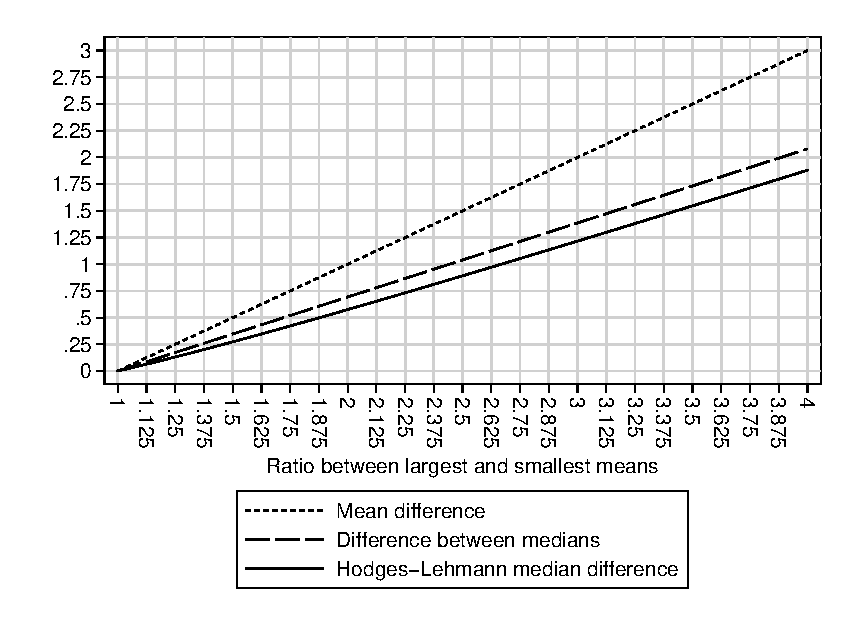
\includegraphics{figseq1.eps}
\end{figure}

\textit{However}, although the median difference and the difference between medians do not converge in difference,
they do converge in ratio.
For $\sigmarat>1$, the ratio between the difference between the medians and the median difference is
\begin{equation}
{{\xi_{0.5}(\Ymaj) - \xi_{0.5}(\Ymin)}\over{\xi_{0.5}(\Ymaj-\Ymin)}}
\quad = \quad
{{\ln(2)}\over{\ln(2) \, - \, \ln(\sigmarat^{-1}+1)}}(1-\sigmarat^{-1}) \, .
\label{eq:eqseq15}
\end{equation}
This is decreasing in $\sigmarat$ where $\sigmarat>1$,
because the numerator and denominator are both zero when $\sigmarat=1$,
and the derivative of the numerator is constant in $\sigmarat$,
and the derivative of the denominator is increasing in $\sigmarat$.
It tends to $2 \ln(2)$ in the limit as $\sigmarat\rightarrow 1$ (by (\ref{eq:eqseq12}) and L'Hospital's rule),
and tends to 1 in the limit as $\sigmarat\rightarrow\infty$.
Therefore, the median difference and the difference between the medians converge in ratio (but \textit{not} in difference),
as the ratio between the means becomes very large.
Figure~\ref{figure:figseq2} shows the ratio as a function of $\sigmarat$ over the domain $1 < \sigmarat \le 4$.

\begin{figure}[tbp]
\caption{Ratio between difference between medians and median difference as a function of $\sigmarat$.}
\label{figure:figseq2}
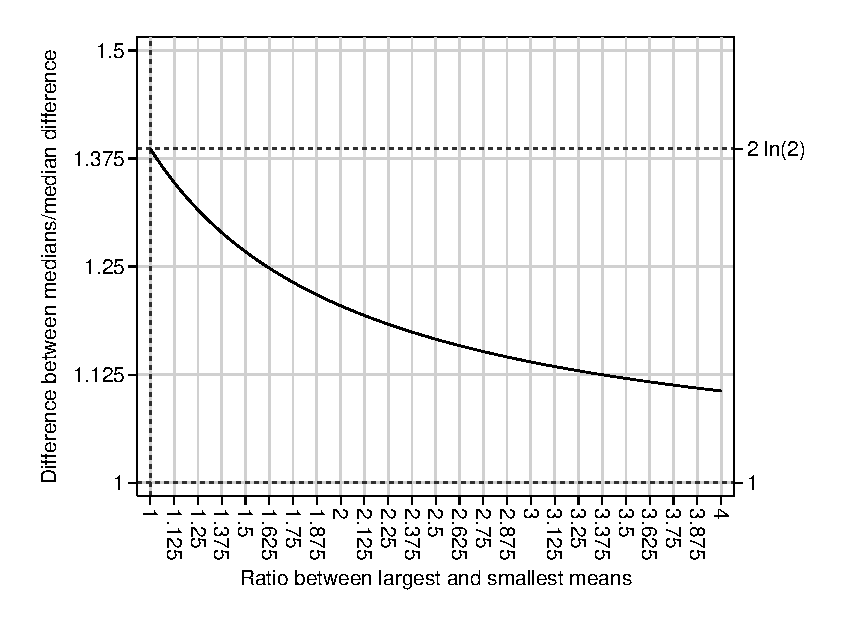
\includegraphics{figseq2.eps}
\end{figure}

\section{References}

{\parindent=0pt

\smallskip

Hodges JL, Lehmann EL. Estimates of location based on rank tests.
\textsl{The Annals of Mathematical Statistics} 1963; \textbf{34(2)}: 598--611.

Lehmann EL. Nonparametric confidence intervals for a shift parameter.
\textsl{The Annals of Mathematical Statistics} 1963; \textbf{34(4)}: 1507--1512.

}

\end{document}               % End of document.
